%%%%%%%%%%%%%%%%%%%%%%%%%%%%%%%%%%%%%%%%%%%%%%%%%%%%%%%%%%%%%%%%%%%%%%%%%%%%%%%%
%2345678901234567890123456789012345678901234567890123456789012345678901234567890
%        1         2         3         4         5         6         7         8

\documentclass[letterpaper, 10 pt, conference]{ieeeconf}  % Comment this line out
                                                          % if you need a4paper
%\documentclass[a4paper, 10pt, conference]{ieeeconf}      % Use this line for a4
                                                          % paper
\usepackage{amsmath}
\usepackage{amsfonts}
\usepackage{float}
\usepackage{graphicx}
\usepackage[colorinlistoftodos]{todonotes}
\usepackage{algorithm}
\usepackage{algpseudocode}
\usepackage{listings}
\usepackage{xcolor}
\usepackage{longtable}
\usepackage{supertabular,booktabs}

\IEEEoverridecommandlockouts                              % This command is only
                                                          % needed if you want to
                                                          % use the \thanks command
\overrideIEEEmargins
% See the \addtolength command later in the file to balance the column lengths
% on the last page of the document



% The following packages can be found on http:\\www.ctan.org
%\usepackage{graphics} % for pdf, bitmapped graphics files
%\usepackage{epsfig} % for postscript graphics files
%\usepackage{mathptmx} % assumes new font selection scheme installed
%\usepackage{times} % assumes new font selection scheme installed
%\usepackage{amsmath} % assumes amsmath package installed
%\usepackage{amssymb}  % assumes amsmath package installed

\title{\LARGE \bf
The Path to DotA 2 Master\\
\large \bf An intelligent model to predict and visualize match result in DotA 2
}

\author{Yuehua Xu$^{1}$, Huanli Wang$^{1}$, Jingfan Sun$^{2}$, Hong Cao$^{1}$, Xueyang Xu$^{2}$% <-this % stops a space
% \thanks{*This work was not supported by any organization}% <-this % stops a space
\thanks{$^{1}$College of Computing, Georgia Institute of Technology, Atlanta, GA 30332 USA}%
\thanks{$^{2}$School of Electrical and Computer Engineering, Georgia Institute of Technology, Atlanta, GA 30332 USA}%
}


\begin{document}

\maketitle
\thispagestyle{empty}
\pagestyle{empty}

%%%%%%%%%%%%%%%%%%%%%%%%%%%%%%%%%%%%%%%%%%%%%%%%%%%%%%%%%%%%%%%%%%%%%%%%%%%%%%%%
\begin{abstract}

People are eager to know the result even before a game begins. So the results prediction is much attractive. DotA 2, the online video game, is widely accepted as a kind of electronic sport program. Our team figures out the correlation between hero selection and winning rates. We then build a web and data-driven system to visualize these results online. Through this system, we apply machine learning methods to train a prediction model by using data from an official, public source and finally draw an conclusion.

\end{abstract}
%%%%%%%%%%%%%%%%%%%%%%%%%%%%%%%%%%%%%%%%%%%%%%%%%%%%%%%%%%%%%%%%%%%%%%%%%%%%%%%%
\section*{NOMENCLATURE}
\subsection*{Terminology}
\begin{supertabular}{p{1.5cm} p{6.4cm}}
DotA 2 & Defense of The Ancients 2\\
hero & The essential element of DotA\\
mode & A set of restrictions within which the game can be played\\
skill & The level of a certain match\\
MidLane & The middle of the three lanes in the map\\
SafeLane & The easier and less risky lane for each faction\\
OffLane & The more risky lane for each faction\\
Jungle & A neutral area between each lane in the map\\
% MOBA & Multiplayer Online Battle Arena games\\
\end{supertabular}
\subsection*{Indices and Sets}
\begin{supertabular}{p{1.5cm} p{6.4cm}}
$S$ & Set of attributes\\
\end{supertabular}
\subsection*{Attribute}
\begin{supertabular}{p{1.5cm} p{6.4cm}}
$a_{bl}$ & The base performance of each hero\\
$a_{ml}$ & The ability of a hero to rival with enemies on MidLane\\
$a_{sl}$ & The ability of a hero to rival with enemies on SafeLane\\
$a_{ol}$ & The ability of a hero to rival with enemies on OffLane\\
$a_{jl}$ & The performance of a hero in Jungle\\
$a_{dps}$ & Initialism for damage per second, a measure of the damage dealt by a hero or unit over one second\\
$a_{p}$ & The ability of a hero to destroy enemy's tower\\
$a_{n}$ & The ability of a hero to deal a large amount of damage in a very short span of time\\
$a_{dur}$ & The ability to take a lot of damage and abuse before dying\\
$a_{i}$ & The ability to take advantage in the early stage of a battle\\
$a_{dis}$ & The ability to impede other heroes' abilities to act\\
$a_{h}$ & The ability to heal teammates\\
$a_{aai}^{ij}$ & Initialism for anti-advantage-index, a higher value means the hero $i$ has a higher advantage over hero $j$\\
$a_{cai}^{ij}$ & Initialism for combo-advantage-index, a higher value means hero $i$ can help hero $j$ better when they are teammates\\
$a_c$ & A measure to evaluate the coordination among allies and advantage among enemies of a specific hero in a team\\
$id$ & The unique index assigned to a past match\\
\end{supertabular}

%%%%%%%%%%%%%%%%%%%%%%%%%%%%%%%%%%%%%%%%%%%%%%%%%%%%%%%%%%%%%%%%%%%%%%%%%%%%%%%%
\section{INTRODUCTION}

The market of E-sports is growing extremely fast. DotA is the most popular one in this area. Essentially an online game, DotA generates a tremendous amount of data from every match played on its servers. Based on these data, we create a mathematical model to predict the winning possibility of each match using the machine learning methods. A web and data-driven system is then built to visualize these results and recommend the optimal combination of heroes to win the game.

Hero selection is an essential part of DotA 2. It is nearly impossible to win without a well coordinated team base. Hero selection is based not only on heroes' attributes but also on their synergy with allied heroes and their performance against enemy heroes. In DotA 2, there are hundreds of heroes and each of them has its own set of strengths and weaknesses, which means mastering selecting heroes is quite challenging. Many teams rely on the experience of players and their impromptu inspiration for matches (selecting heroes). However, most ordinary players do not have such talent and this limits their performance. With the help of our proposed system, a rookie is able to test different team bases online and finally gain experience from doing comparisons. 

This paper is structured as follows:  Section II summaries previous work in this area, Section III briefly describes the game mechanism of DotA 2, and Section IV introduces data collected and pre-processing of data. In Section V, the structure of proposed system is presented. Details about the match prediction model can be found in section VI. Thereafter, we are able to predict the winning probability of any combination of heroes. The model is trained and tested under various situations. Results and Summary of Innovations are shown in section VII and section VIII, respectively. Finally, conclusions are drawn in Section IX.

\section{SURVEY}
In recent years, there has been a number of publications to predict game results in different domains, including traditional sports and E-sports. 

Various ideas have been come up with to predict traditional sport games results. Cao[1] used an SVM, naïve Bayes, and a multilayer perceptron neural network to predict basketball game results. Kahn[2] proposed a multilayer perceptron neural network to predict football results. Trawinski[3] considered the prediction problem as a binary classification. He designed a fuzzy model to predict ACB league results by using a three-phase modeling process. Buursma[4] selected a set of features and used a number of classification algorithms including simple and logistic regression, Bayesian network, naïve Bayes, and decision tree to predict soccer match results.

In the DotA 2 domain, Song et al[5] used Logistic regression to predict winning side based on hero lineups, but the result was not satisfying given the inadequacy of factors which was taken into account. Kinkade[6] proposed two win predictors for DotA 2 analysis. One of them used full post-match data and the other used only hero selection data. Neidhardt et al.[7] explored the impacts of different types of team factors on performance (like Team Ecosystem Factors, Team Process and Duration and etc), which are compositional, relational and ecosystem factors. Conley et al.[8] presented a hero recommendation engine, detailed with method of data collection and features selection. An augmentation algorithm was presented by Kalyanaraman[9] to predict the outcome of DotA 2 matches and recommend the hero lineups.

Some researches focus on spatio-temporal behaviors across four skill tiers and two measures: zone changes and intra-team distance[10] in order to analyze team behaviors. Eggert et al.[11] used the logistic regression to classify players' behavior based on attributes they constructed from replay files. Pobiedina et al.[12][13] investigated that to which extent different factors of the team in the game, such as role distribution, experience, number of friends and national diversity, have influences on the team's success.

If game-state data can be collected real-timely from the game APIs, it is possible to perform a machine learning algorithm to predict the result of an ongoing DotA 2 game as it is progressing. DotA 2 provides a powerful replay system which preserves almost all necessary information. That is, replays of the DotA 2 can be used as the training dataset. Features and patterns extracted from replays will help to create the model of result prediction. Johansson and Wikström[14] performed several algorithms to different models and the Random Forest came out as the most accurate one.

\section{DEFENCE OF THE ANCIENTS 2}

Defense of the Ancients 2 (DotA 2)[19] is a Free-to-Play (F2P) game that originated from the DotA mod of Warcraft 3: Reign of Chaos which was released in 2003.The mod became popular and supported a substantial e-sports scene.[18] By 2009, Valve began developing DotA 2 as a standalone game. It went into beta testing in 2011. DotA 2 is today the most played game on the online distribution platform Steam, in itself on of the most heavily trafficked digital game platforms in the world. DotA 2 also hosts the biggest prize pools in e-sports. Furthermore, the game has a reported number of 7.86 million of monthly active players and achieved a revenue of 80 million USD in 2013 via micro-transactions which are limited to selling cosmetic items.[17]

\begin{figure}[h]
\begin{center}
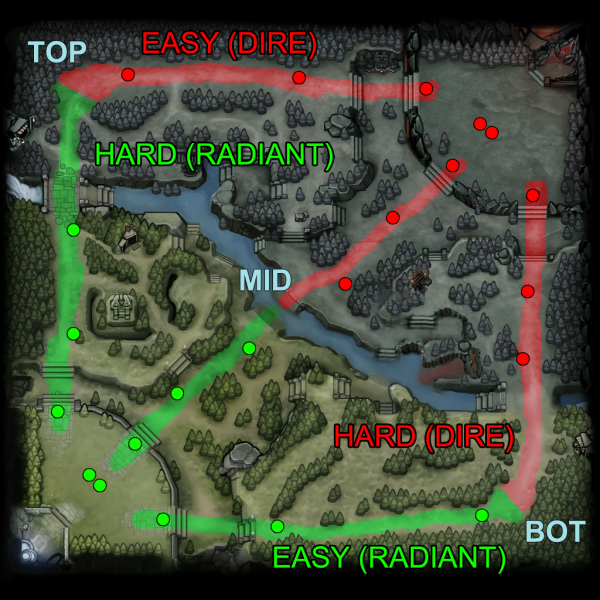
\includegraphics[width=0.4\textwidth]{600px-Minimap_Lanes.png}
\caption{The DotA 2 map. The Radiant base is at the bottom left, the Dire base at the top right.}
\end{center}
\end{figure}

\subsection{Game Process}
DotA 2 is played by two teams of 5 players, each of them controlling one avatar-character being selected from a roster of 112 predefined heroes. Each hero has different abilities and is suited for different roles in the game, e.g. for dealing damage at a distance. Each hero can gain levels similar to an archetypical character in a Role-Playing Game. Additionally, a hero can be equipped with a variety of objects that improve the characters base statistics or increase, alter or add new abilities. Items are bought with gold being earned during the game, e.g. from killing other player’s characters, creeps or towers (see below). Experience to level up characters and thereby unlock better versions of the hero’s abilities or new abilities, is earned in a similar way. Tactics and strategy are key components in the game, and communication between team members is very important. Players can communicate via text chat, voice chat, alert messages in the arena itself (“pings”) or by writing on the minimap.The game is viewed from an isometric perspective. Games have no time limit, but the matches used in the current work average about 40 minutes in length. The two teams compete in a geographically balanced, square virtual arena, and the same arena is used in every match. The arena is split in two parts, with each half owned by one team at the beginning of a match (Figure 2). The arena contains a variety of game-related features, most importantly a base for each team with a central building, the ancient, which the opposing team must destroy to win. The ancients are guarded by a series of defensive structures called towers which provide defensive capabilities. Additionally, the two bases regularly spawn computer-controlled units called creeps which rush the opposing team’s towers and players. The presence of towers and creeps results in an unstable balance that oscillates slowly [5]. There are three main pathways through the map, referred to as lanes (Figure 1). These are differentiated “top”, “middle”, and “bottom”. The lanes form vital strategic points of attack on the opposing team’s defences. However, there are a variety of sub-environments in the DotA 2 environment, which sees different tactical and strategic uses. For example, the jungle area in between the lanes form a means for levelling up a hero via killing regularly re-spawning computer-controlled neutral units, as well as for launching surprise attacks on enemy players or creeps.

\section{DATA AND PRE-PROCESSING}

The quality of dataset is essentially important for training  of prediction model. The dataset we used can be divided into three parts: 
\begin{enumerate}
\item Hero attributes
\item Advantage indices
\item Historical match data
\end{enumerate}
Among these three, both \textit{Hero attributes} and \textit{Historical match data} are both raw data and are available online. A \texttt{Python} script is written to acquire these data from \textit{DotA 2 API} \cite{c1}. \textit{Advantage indices} is a secondary dataset which is processed and  calculated based on \textit{Hero attributes}. Detailed description can be found below.
\subsection{Hero attributes}
There are 112 heroes included in our analysis. Each hero has two set of attributes (The meaning of these attributes can be found in NOMENCLATURE).
\begin{itemize}
\item Lane Attributes: $\{a_{bl}, a_{ml}, a_{sl}, a_{ol}, a_{jl}\}$
\item Battle Attributes: $\{a_{dps}, a_{p}, a_{n}, a_{dur}, a_{i}, a_{dis}, a_{h}\}$
\end{itemize}
The range of both \textit{Lane Attributes} and \textit{Battle Attributes} are from $0$ to $10$. The higher the value, the higher the performance of that hero on this certain attribute.

\subsection{Advantage indices}
Based on \textit{Hero attributes}, we introduce two indices \textit{anti-advantage-index} and \textit{combo-advantage-index} for each hero pair $\{\text{Hero }i, \text{Hero }j\}$.
$$a_{aai}^{ij}=\frac{\text{Average winning rate when } i \text{ and } j \text{ are enemy}}{\text{Average winning rate of }i}$$
$$a_{cai}^{ij}=\frac{\text{Average winning rate when } i \text{ and } j \text{ are teammates}}{\text{Average winning rate of }i}$$
In this way, we create two $112\times 112$ matrices, \textit{anti-advantage-index-matrix} and \textit{combo-advantage-index-matrix}. The entry on $i$th row and $j$th column of each matrix is the \textit{anti-advantage-index} $a_{aai}^{ij}$ and \textit{combo-advantage-index} $a_{cai}^{ij}$ of this hero pair $\{\text{Hero }i, \text{Hero }j\}$ respectively. 
% $a_{aai}$ & Initialism for anti-advantage-index, a higher value means the first hero has a higher advantage over the second hero\\
% $a_{cai}$ & Initialism for combo-advantage-index, a higher value means the first hero can help the second hero better when they are teammates\\

\subsection{Historical match data}
There are over $2.7$ billion historical matches data available online. We collected $100$ thousand matches for model training. Each \textit{Historical match data} has $12$ entries \{$id$, $result$, \{\text{five heroes of first team}\}, \{\text{five heroes of second team}\}\}. $id$ is the unique index assigned to a past match. $result$ is either $0$ or $1$, which indicates "win" or "lose".


\section{Structure of Proposed System}

Figure. 2 is the general structure of the proposed web and data-based system. The whole system are divided into two major subsystems, Training Subsystem and Web-Analysis Subsystem.

\begin{figure}[h]
\begin{center}
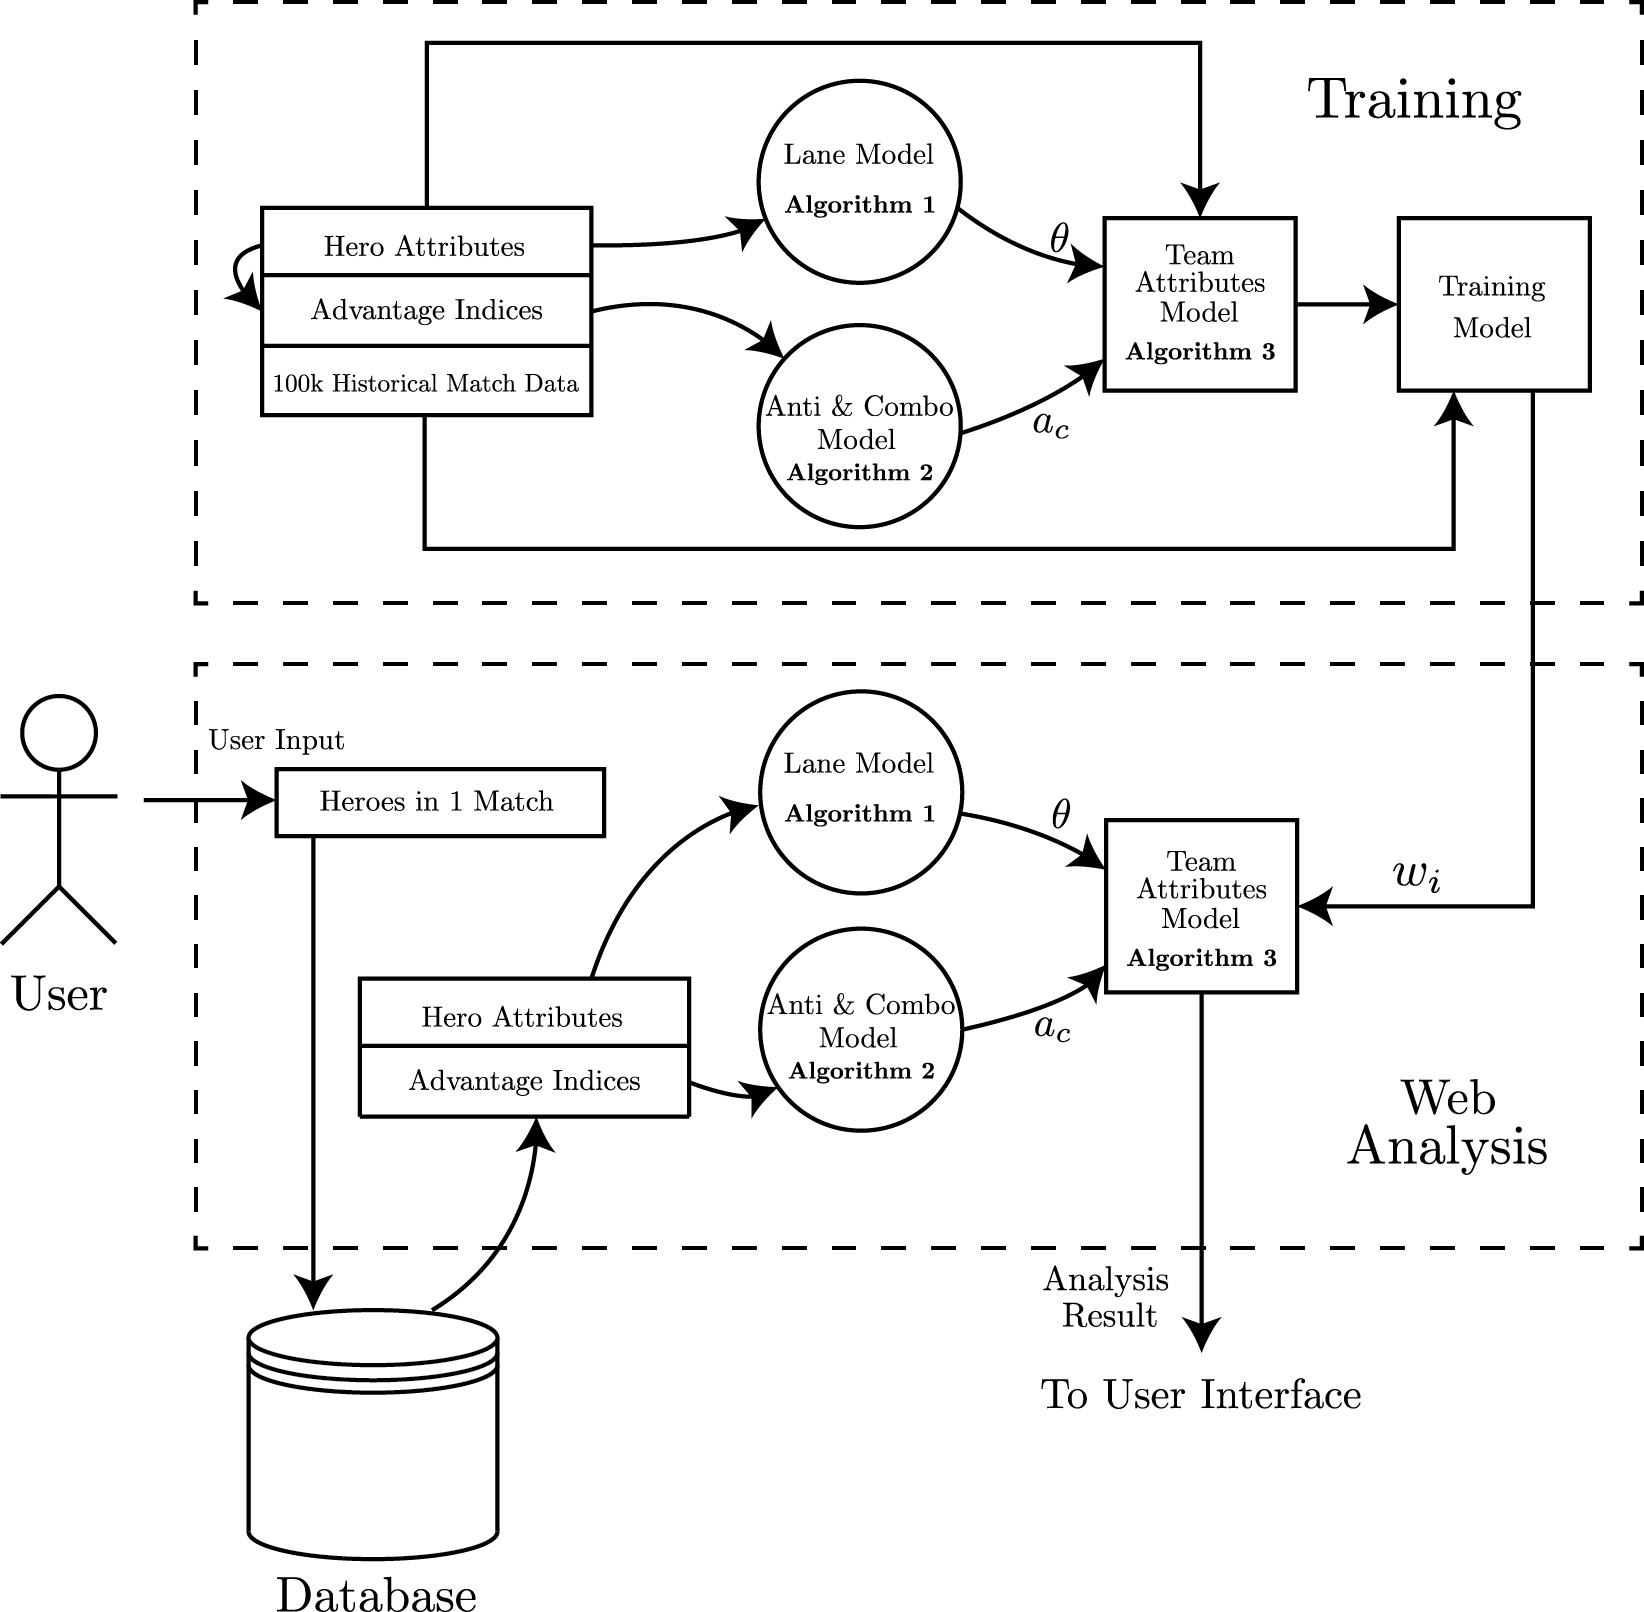
\includegraphics[width=0.47\textwidth]{6242big_picture.png}
\caption{Detailed structure of proposed web and data-based system}
\end{center}
\end{figure}

\subsection{Training Subsystem}
Based on the data collecting and pre-processing method from Section IV, we generate \textit{Hero attributes}, \textit{Advantage indices}, and collected \textit{Historical match data} from $100k$ matches in total. These datasets (at top-left side in Figure. 2) form the foundation for match prediction algorithms proposed in Section VI.

In Training subsystem, dataset \textit{Hero attributes} and \textit{Advantage indices} are sent to \textbf{Lane Model (Algorithm 1)} and \textbf{Anti \& Combo Model (Algorithm 2)}, respectively. The output of these two models are Resource-Adjustment-Index $\theta$ and Advantage-Adjustment-Index $a_c$. These two parameters, along with dataset \textit{Hero attributes} itself, are sent to \textbf{Team Attributes Model (Algorithm 3)}. 

The subsystem is then trained based on the output of \textbf{Algorithm 3} and $100k$ \textit{Historical match data}. Finally, we obtain weighted parameters $w_i$ for each model attributes. These weighted parameters are used to calculate analysis results (winning rate, etc.) in Web-Analysis subsystem.

\subsection{Web-Analysis Subsystem}

The Web-Analysis subsystem is an interface between website users and our proposed prediction model. A screen shot of the website \footnote{http://believerw.github.io/ThePathToDotAMaster/index.html} is presented in Figure. 3.
\begin{figure}[h]
\begin{center}
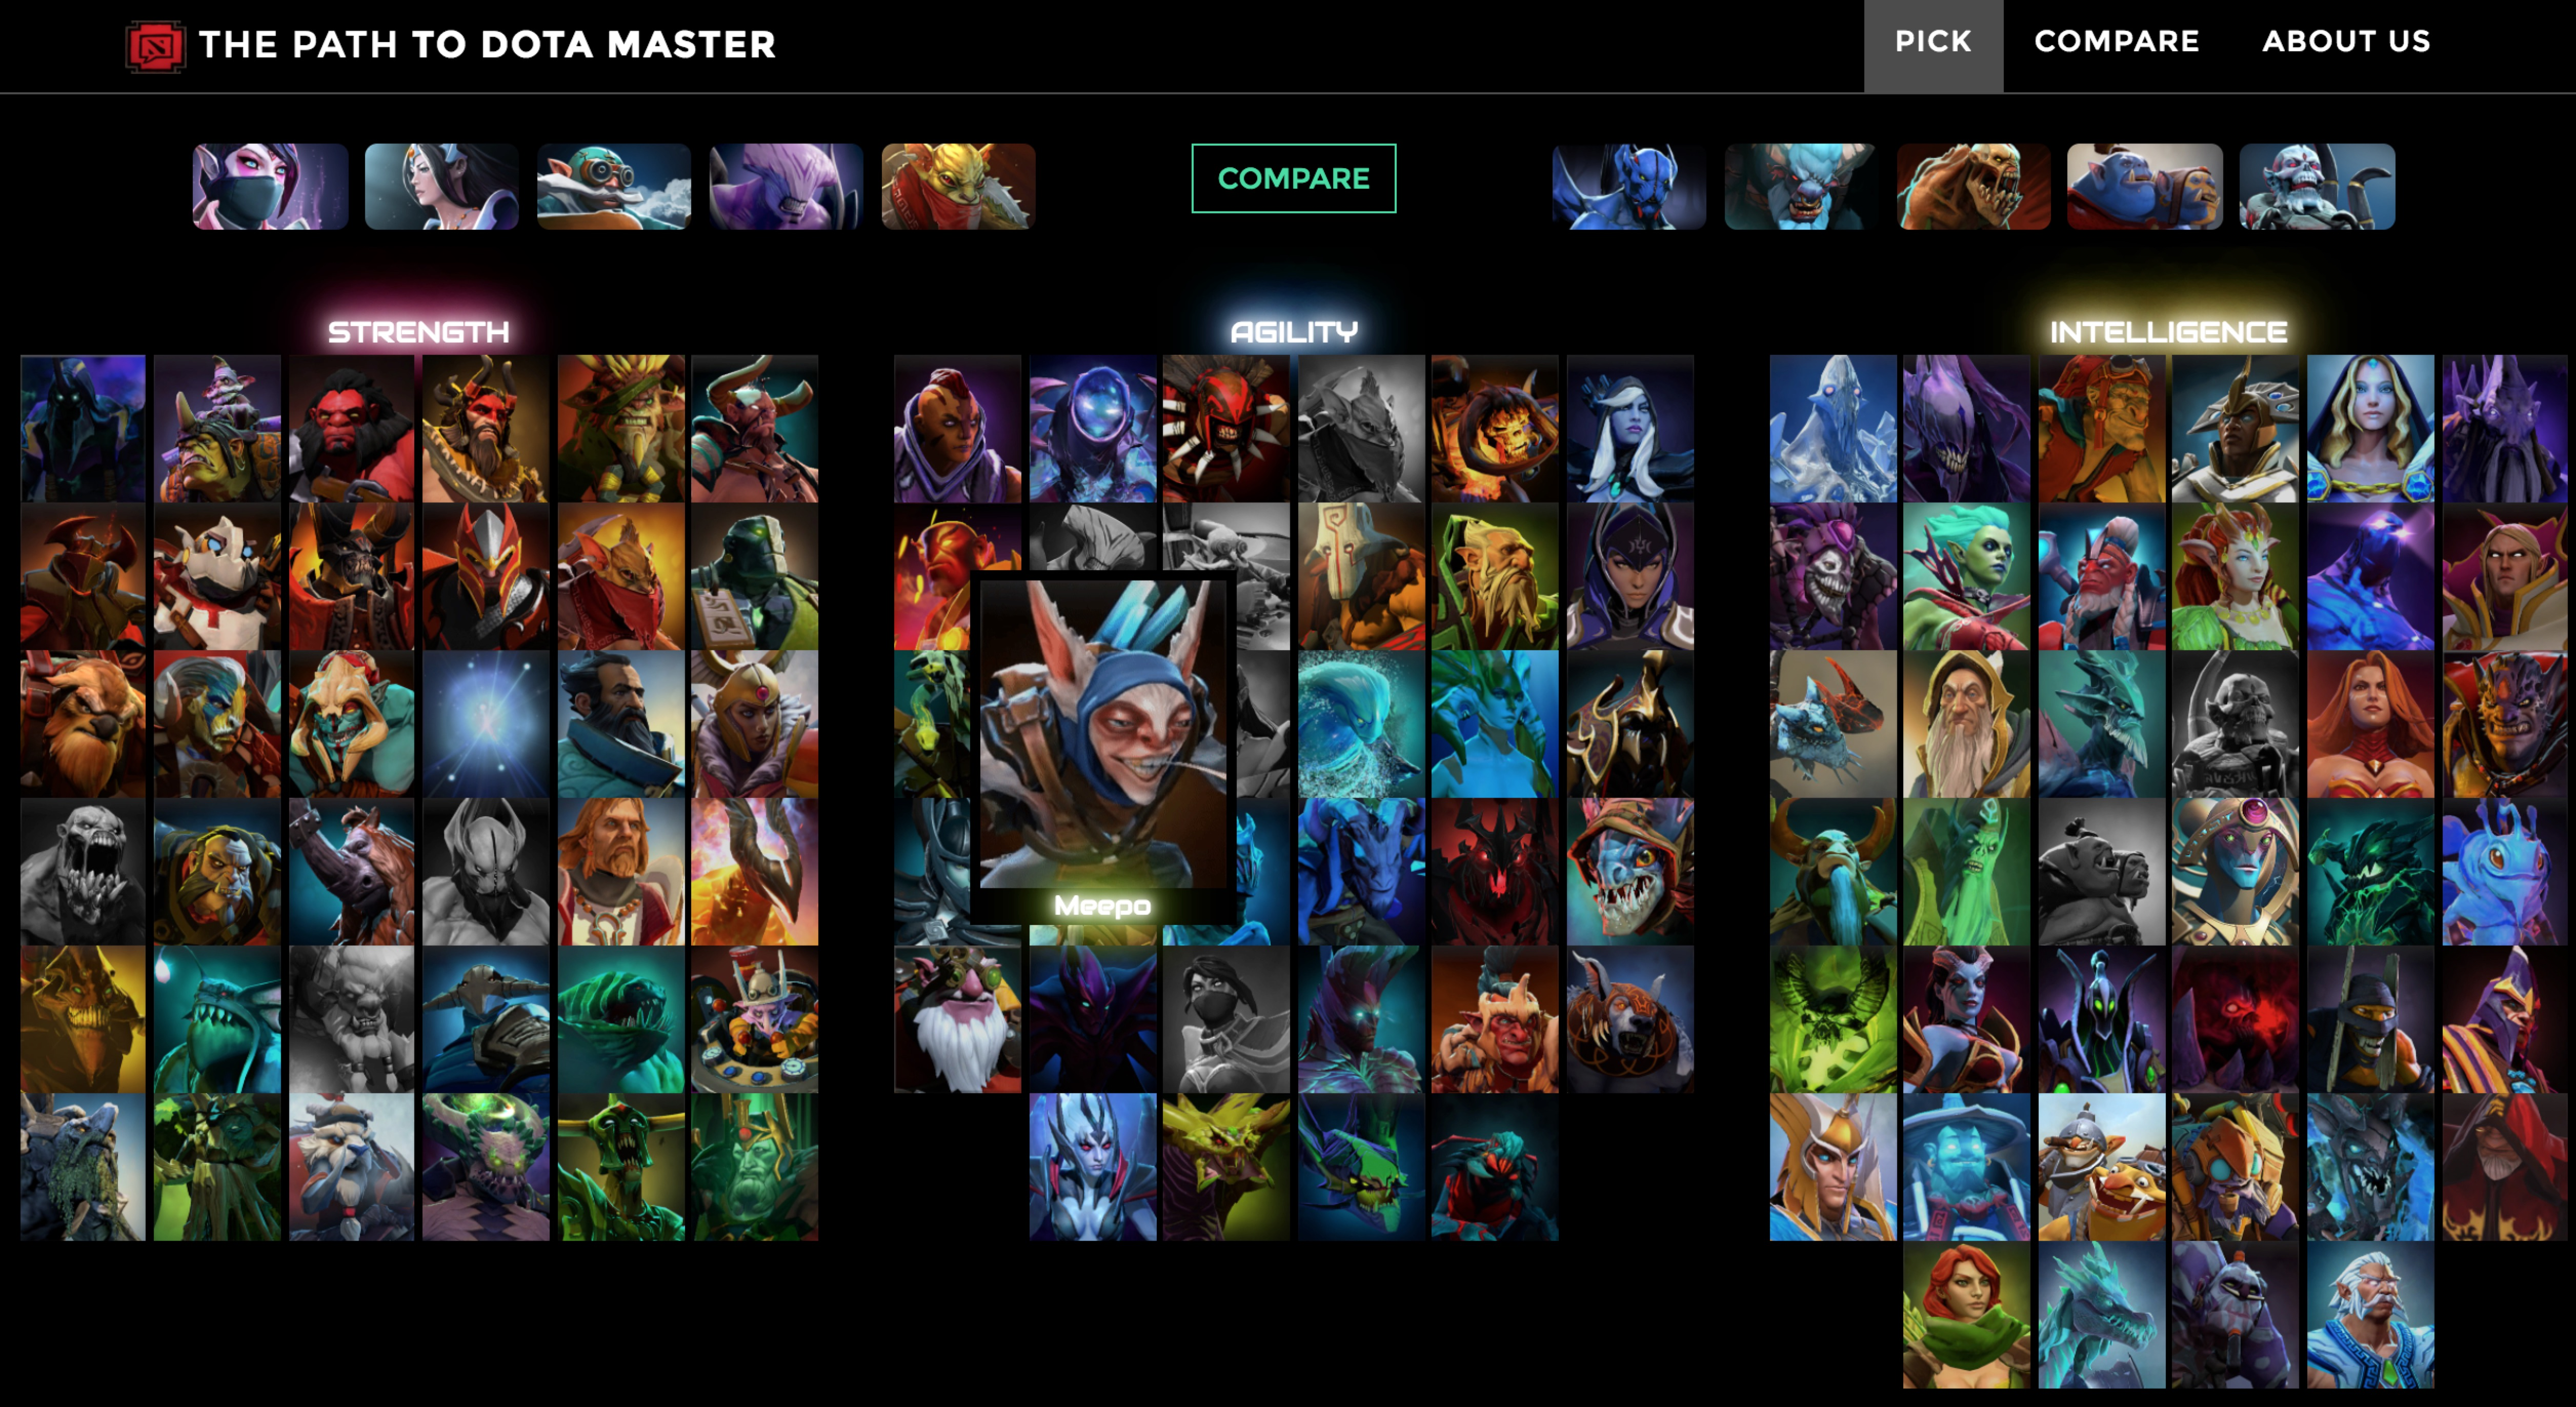
\includegraphics[width=0.45\textwidth]{pick.jpg}
\caption{A screen shot of user interface on the website for web analysis subsystem. \textit{url: http://believerw.github.io/ThePathToDotAMaster/index.html}}
\end{center}
\end{figure}

Datasets \textit{Hero attributes} and \textit{Advantage indices} are stored in a database (bottom-left corner of Figure. 2). Whenever a website user enters the 10 hero names of both teams, subsystem searches in the database and selects all the attributes related to these 10 heroes. These attributes are sent to \textbf{Lane Model (Algorithm 1)} and \textbf{Anti \& Combo Model (Algorithm 2)} which are fast enough to be implemented in the web analysis. Combined with the pre-trained weighted parameters $w_i$, we are able to calculate all the results needed from \textbf{Team Attributes Model (Algorithm 3)}. Later, Web-Analysis subsystem performs a data visualization on the user interface and users can read it directly from the website.

\section{MATCH PREDICTION MODEL}

Basically, strength of each team base is modeled as a Gaussian distribution. 
$$f_1(x|\mu_1, \sigma_1^2) = \frac{1}{\sqrt{2\sigma_1^2 \pi}} e^{-\frac{(x-\mu_1)^2}{2\sigma_1^2}} $$
$$f_2(x|\mu_2, \sigma_2^2) = \frac{1}{\sqrt{2\sigma_2^2 \pi}} e^{-\frac{(x-\mu_2)^2}{2\sigma_2^2}} $$
where $\mu_1$ and $\mu_2$ represent the average strength of each team while $\sigma_1$ and $\sigma_2$ models the stability of performance. After obtaining these parameters from training algorithm, we are able to calculate the difference of these two distributions. The result we get is also a Gaussian distribution which we denote as $f_3(x|\mu_3, \sigma_3^2)$.
$$f_3(x|\mu_3, \sigma_3^2) = \frac{1}{\sqrt{2(\sigma_1^2 + \sigma_2^2) \pi}} e^{-\frac{(x-(\mu_1-\mu_2))^2}{2(\sigma_1^2 + \sigma_2^2)}} $$

Then, we calculate the \texttt{cdf} of $f_3$ and name it $g_3$. The value at $x = 0$ is the winning rate (possibility of winning) of second team. For example, in Figure. 4, we provide a set of typical values for $f_1$ and $f_2$. 
$$f_1: \mu_1 = 7.34, \sigma_1 = 47.74$$
$$f_2: \mu_2 = -4.42, \sigma_2 = 42.58$$
$$f_3: \mu_3 = 11.76, \sigma_3 = 64.49$$
\begin{figure}[h]
\begin{center}
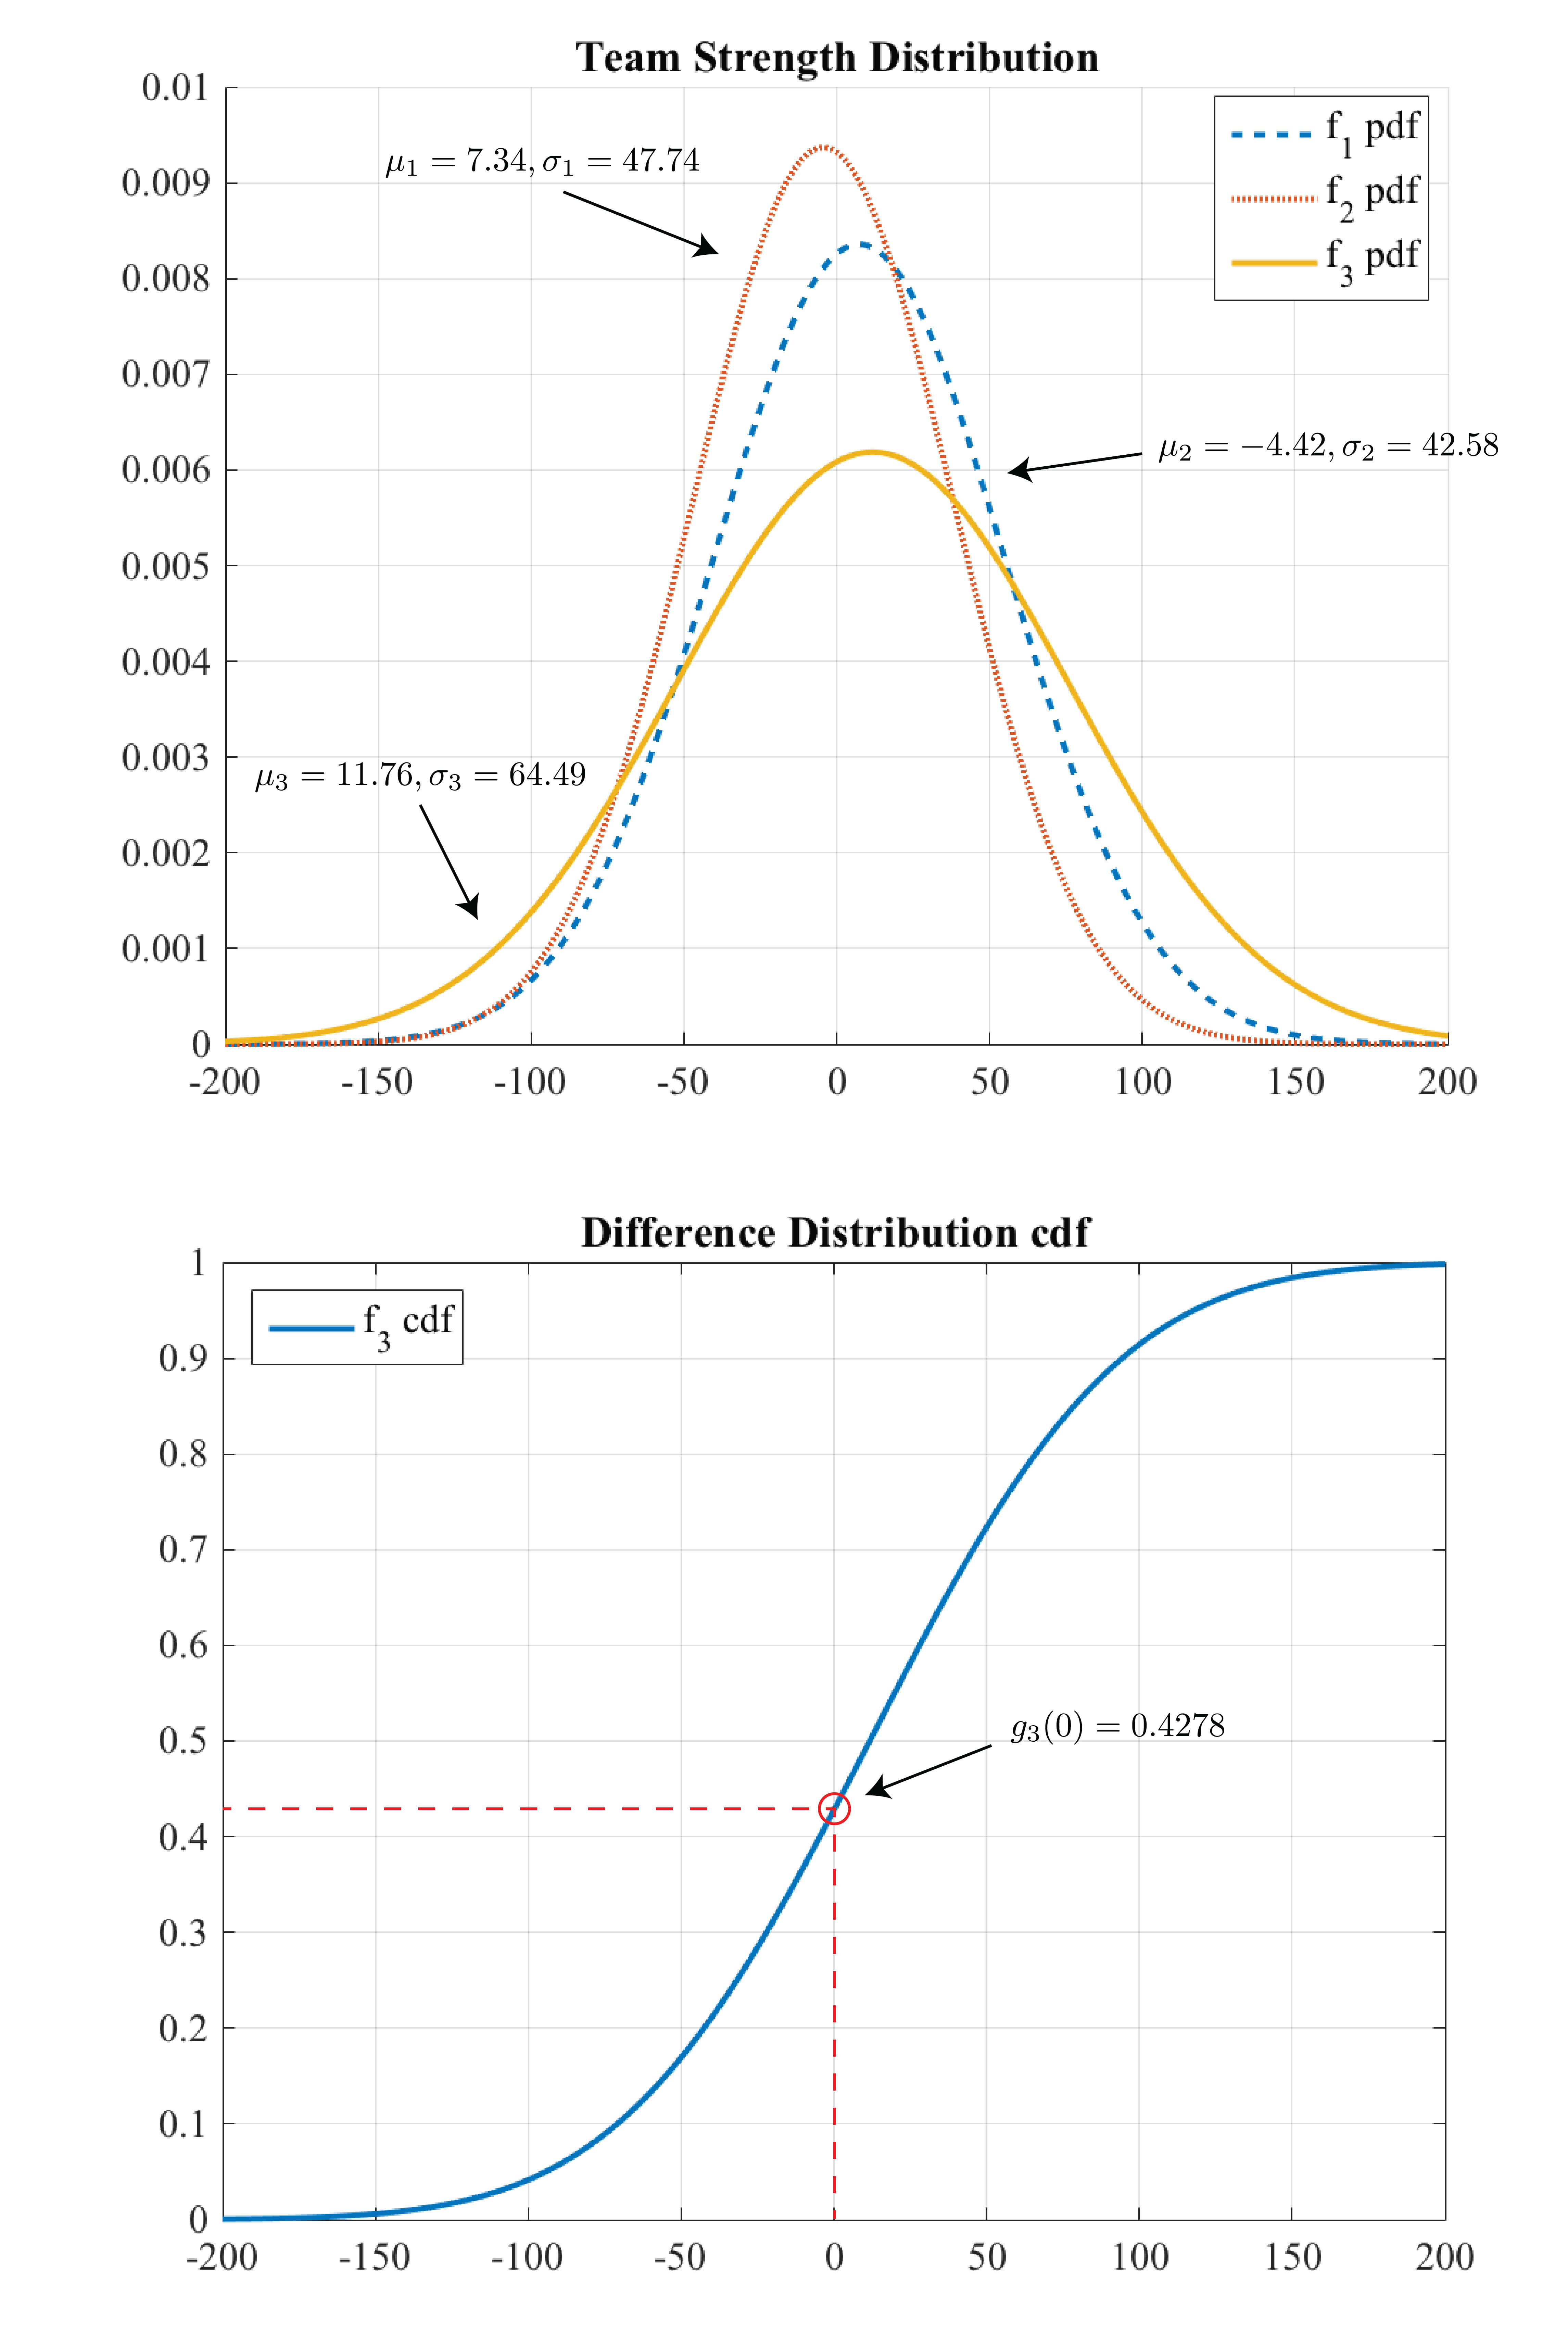
\includegraphics[width=0.45\textwidth]{distribution_ai.png}
\caption{Team strength distribution}
\end{center}
\end{figure}

Based on Figure. 4, we find $g_3(0) = 0.4278$. It means the winning rate of second team is $42.78\%$, the winning rate of first team is $100\% - 42.78\% = 57.22\%$.

Now, we describe the training algorithms in detail. There are mainly three algorithms used in match prediction model, Lane Model (Algorithm 1), Anti \& Combo Model (Algorithm 2) and Team Attributes Model (Algorithm 3).

\subsection{Lane Model}

In DotA 2, the performance of a hero is greatly impacted by resource. However, the dataset \textit{Hero attributes} only has the data of heroes in normal resource situation. To improve the accuracy of prediction model, we introduce the Lane Model with which we can show the level of resource by a Resource-Adjustment-Index $\theta$. 

\begin{algorithm*}
\caption{Lane Model}
\begin{algorithmic}
\Function{lane cmp}{$radiant, dire$}
    \For{$side$ in $radiant, dire$}
        \If{side has at least one hero perfer MidLane}
            \State Find the hero with max ability in MidLane with preference of MidLane: $M$
        \Else
            \State Find the hero with max ability in MidLane and time decay rate 0.85: $M$
        \EndIf
        \If{there are hero in jungle}
            \State Find the hero with  max ability in jungle: $J$
            \State Find the hero with  max ability in OffLane and time decay rate 0.7: $O$
            \State Set the other two heroes in SafeLane and get the sum of abilities in SafeLane: $S$
            \State Get the general ability with hero in jungle of $side$: $L_1 = (M+J+O+S)/5$
        \Else
            \State find the max sum ability of two heroes in SafeLane and two heroes in OffLane: $S$
            \State Get the general ability with hero in jungle of $side$: $L_2 = (M+S)/5$
        \EndIf
        \State $L[side] = max(L_1, L_2)$ 
    \EndFor
\State $\theta = 2 / (1 + exp((L[dire] - L[radiant]) / \alpha))$
\EndFunction
\end{algorithmic}
\end{algorithm*}

As is shown in \textbf{Algorithm 1}, we get the base performance data for heroes in both teams first. After training the weight $\alpha$, we perform an optimization and calculate the $\theta$ we need. $\theta$ is in a range of $[0, 2]$. The higher the $\theta$, we higher the adjustment for team 1. For example, a $\theta = 1.2$ means that the performance of team 1 will be strengthened by a factor of 1.2 because they have better resource. On the contrary, the performance of team 2 is weaken by $2 - 1.2 = 0.8$ because the lack of resource limits their abilities. 

\begin{figure}[H]
\begin{center}
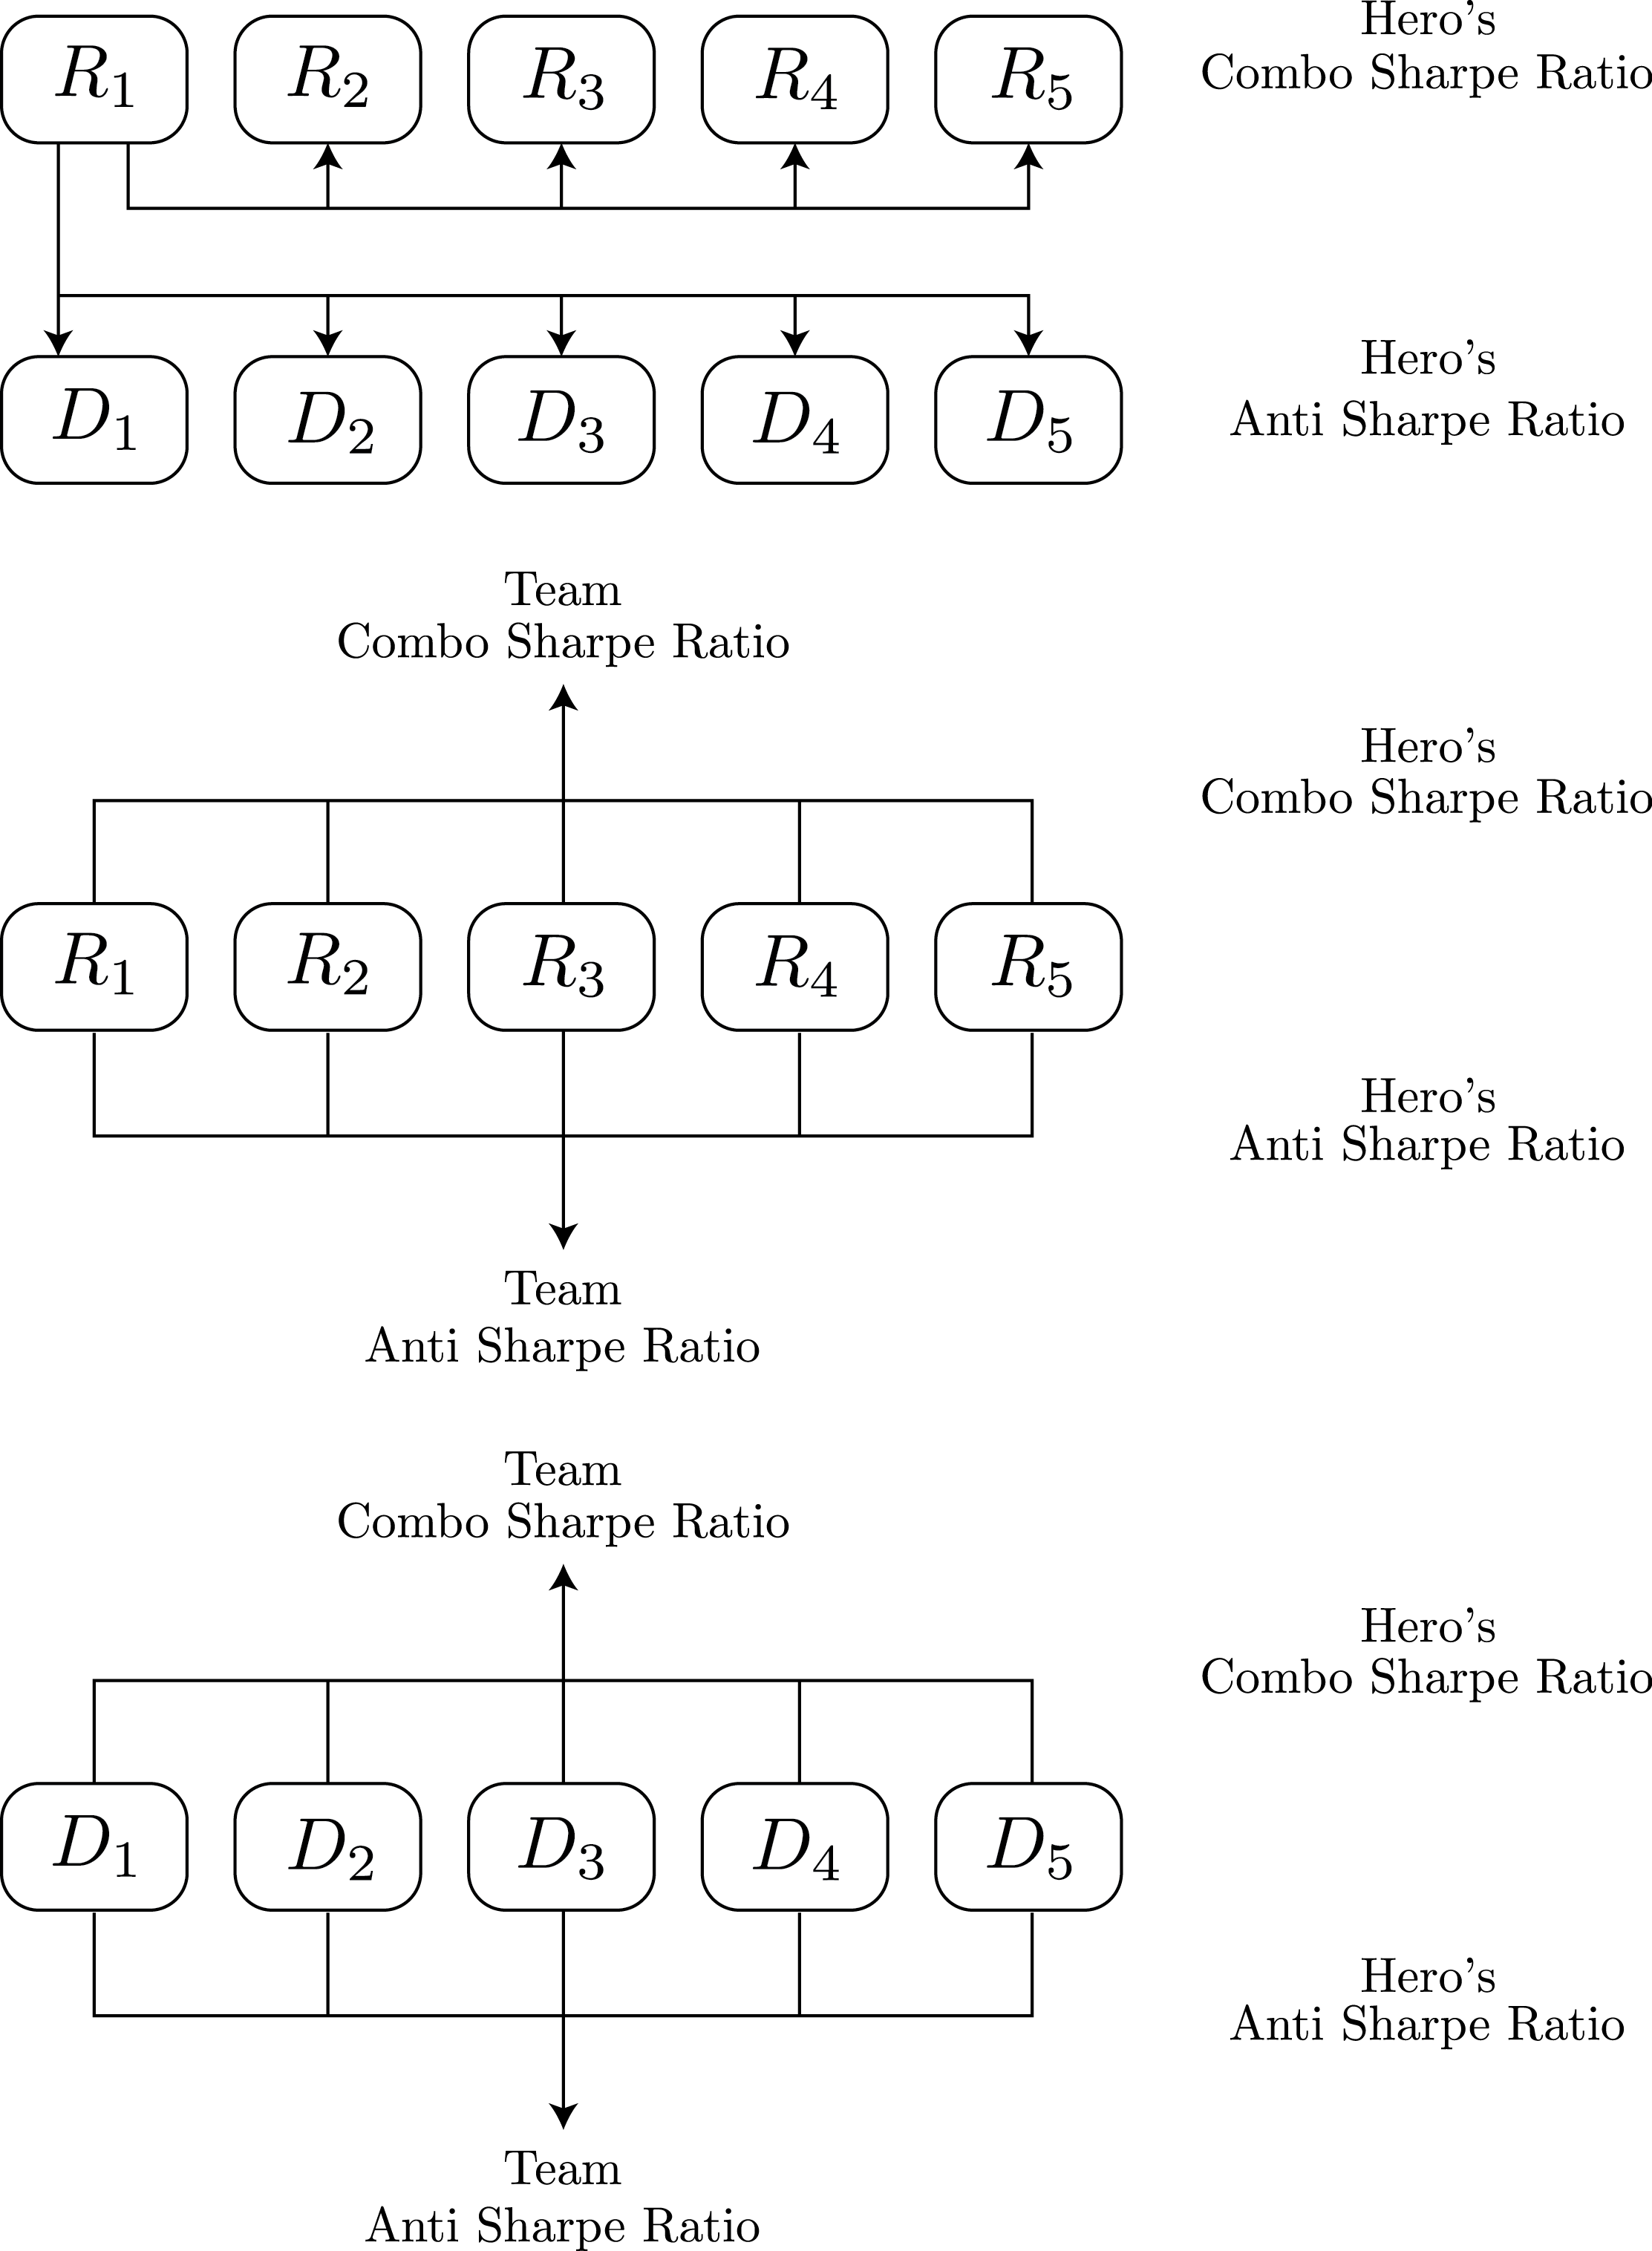
\includegraphics[width=0.45\textwidth]{sharpe_ratio.png}
\caption{Sharpe ratio calculation Demonstration}
\end{center}
\end{figure}

\subsection{Anti \& Combo Model}

The data from dataset \textit{Hero attribute} measures the performance of a hero in a standalone mode. However, in a real DotA game, heroes are grouped into two teams and therefore, apparently, their performance is significantly influenced by their teammates and enemies. Anti \& Combo Model (Algorithm 2) is presented here to take this influence into consideration.

The idea comes from \textit{"Sharpe Ratio"} which is a terminology widely used in finance analysis. It is a way to examine the performance of an investment by adjusting for its risk. In our model, we use the same idea to calculate the \textit{"Sharpe Ratio"} for \textit{anti-advantage-index} and \textit{combo-advantage-index}.

In the second part of our dataset, we have \textit{Advantage indices}. This is two $112 \times 112$ matrices where element$[i][j]$ represents the \textit{anti-advantage-index} $a_{aai}^{ij}$ and \textit{combo-advantage-index} $a_{cai}^{ij}$ of a hero pair $\{\text{Hero }i, \text{Hero }j\}$ respectively. We use $R$ and $D$ to denote the two teams. Thus, the heroes in both teams are ${R_1, R_2, R_3, R_4, R_5}$ and $D_1, D_2, D_3, D_4, D_5$, respectively. 

Figure. 5 is an illustration showing how to calculate \textit{"Sharpe Ratio"} in our case. We use $R_1$ as an example. $R_1$ has 4 teammates, its \textit{Combo Sharpe Ratio} is 
$$R_1's\text{ Combo Sharpe Ratio} = \frac{E\{R_2, R_3, R_4, R_5\}}{\sigma{\{R_2, R_3, R_4, R_5\}}}$$
where $E\{R_2, R_3, R_4, R_5\}$ is the expectation and $\sigma{\{R_2, R_3, R_4, R_5\}}$ is the standard deviation. 

Similarly, $R_1$ has 5 enemies, its \textit{Anti Sharpe Ratio} is 
$$R_1's\text{ Anti Sharpe Ratio} = \frac{E\{D_1, D_2, D_3, D_4, D_5\}}{\sigma{\{D_1, D_2, D_3, D_4, D_5\}}}$$

After repeating this method for all 10 heroes in two teams, we have both \textit{Hero's Combo Sharpe Ratio} and \textit{Hero's Anti Sharpe Ratio} for every hero. It is totally 20 sharpe ratios. Then we go ahead to compute \textit{Team Combo Sharpe Ratio} and \textit{Team Anti Sharpe Ratio}. Let's take \textit{Team Combo Sharpe Ratio} of Team R as an example.
$$\text{Team R Combo Sharpe Ratio}$$ 
$$= \frac{E\{CSR_{R_1}, CSR_{R_2}, CSR_{R_3}, CSR_{R_4}, CSR_{R_5}\}}{\sigma{\{CSR_{R_1}, CSR_{R_2}, CSR_{R_3}, CSR_{R_4}, CSR_{R_5}\}}}$$
where $CSR_{R_1}, CSR_{R_2}, CSR_{R_3}, CSR_{R_4}, CSR_{R_5}$ are \textit{Combo Sharpe Ratio} for hero $R_1, R_2, R_3, R_4, R_5$, respectively.



Finally, we have \textit{Team Combo Sharpe Ratio} and \textit{Team Anti Sharpe Ratio} for each team. The advantage-adjustment-index $a_c$ is then computed with the algorithm shown in Algorithm 2.

\begin{algorithm}
   \caption{Anti\&Combo Model}
    \begin{algorithmic}
      \Function{anti\_combo}{$radiant, dire$}

        \For{$side$ in $radiant, dire$}
            \For{$hero$ in $side$}
                \State get the sharpe ratio of the anti-advantage index
                \State $\quad$ of $hero$ with 5 enemy heroes: $A[side][hero]$
                \State get the sharpe ratio of the combo-advantage
                \State $\quad$ index of $hero$ with 4 allay heroes:
                \State $\quad C[side][hero]$
            \EndFor 
        \State get the sharpe ratio of $A[side]$
        \State get the sharpe ratio of $C[side]$
        \State $sr[side] = A[side]+C[side]$
        \EndFor
        \State $a_c = sr[radiant]-sr[dire]$
     \EndFunction
\end{algorithmic}
\end{algorithm}

\subsection{Team Attributes Model}

In a normal DotA match, among the 5 heroes in a team, different hero plays different roles. Some of them are good at dealing damage, while some of them are specialized in healing their teammates. 

Form this perspective, to optimize the performance of a team, we can just take a weighted average of the 5 members to calculate the team attributes. For example, among the 5 heroes $R_1, R_2, R_3, R_4, R_5$, $R_1$ and $R_2$ are good at attacking. Therefore, their weights on attribute $a_{dps}$ will be higher then their teammates. As is shown in Figure. 6, with this average method, we obtain the 11 attributes for each team. 
$$\{a_{bl}, a_{ml}, a_{sl}, a_{ol}, a_{jl}, a_{dps}, a_{p}, a_{n}, a_{dur}, a_{i}, a_{dis}, a_{h}\}$$

\begin{figure}[H]
\begin{center}
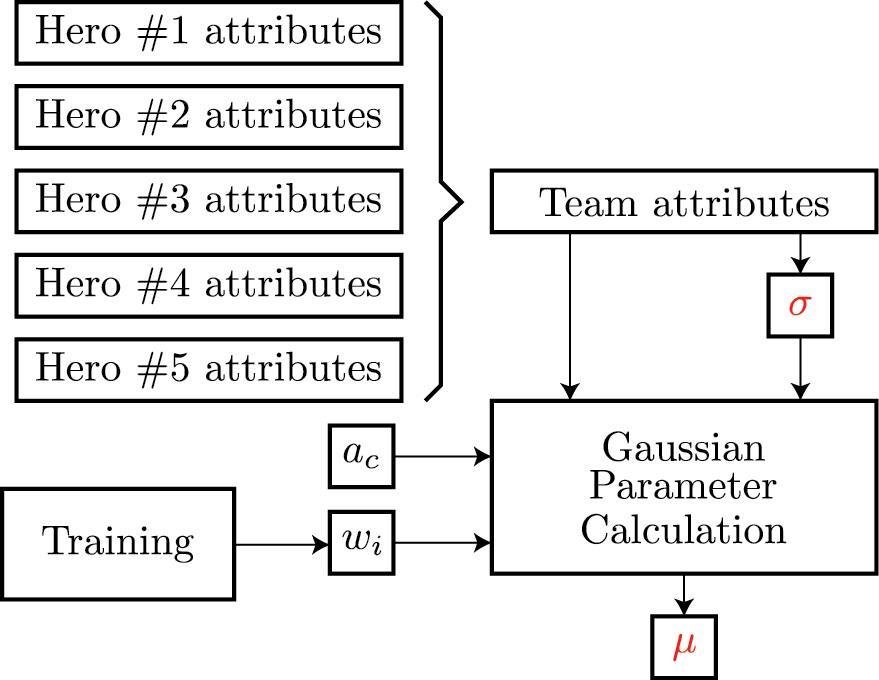
\includegraphics[width=0.45\textwidth]{team_attribute.png}
\caption{Detailed process of Team Attributes Model}
\end{center}
\end{figure}

The next step is to calculate $\mu$ and $\sigma$ for the Gaussian model mentioned at the beginning of this section. 
$$\sigma = std\{a_{bl}, a_{ml}, a_{sl}, a_{ol}, a_{jl}, a_{dps}, a_{p}, a_{n}, a_{dur}, a_{i}, a_{dis}, a_{h}\}$$

As for $\mu$, we add two parameters $\sigma$ and $a_c$ into our 11 attributes set. Thus, we have 13 attributes in total. After training $w_i$ (details presented in next subsection), we can calculate $\mu$ as followed. 
$$\mu = \frac{1}{13}\Sigma_{i = 0}^{13}w_i A_i$$
where $w_i$ is the weight and $A_i$ is the $i$th attribute in set 
$$\{a_{bl}, a_{ml}, a_{sl}, a_{ol}, a_{jl}, a_{dps}, a_{p}, a_{n}, a_{dur}, a_{i}, a_{dis}, a_{h}, a_c, \sigma\}$$

Therefore, in \textit{Team Attributes Model}, we are able to obtain $\mu$ and $\sigma$ for Gaussian Distribution of each team. The winning rate of any combination of heroes can be computed then. Algorithm 3 shows the details regarding how to calculate these team attributes. 

\begin{algorithm}
\caption{Team Attributes Model}
\begin{algorithmic}
\Function{team\_attributes}{$radiant, dire$}
    \For{$side$ in $radiant, dire$}
        
        \For {$attribute$ in $attributes$}
            \If{$attribute$ is $disable$}
                \State weight: $w = [1, 1, 1]$
            \ElsIf{$attribute$ is $initial$ or $healing$}
                \State weight: $w = [0.7, 0.3]$
            \Else
                \State weight: $w = [1.5, 1.5, 1.1, 0.2, 0.2]$
            \EndIf
            \State sort the $attribute$ of $hero$ in $side$ by 
            \State $\quad$ descending and get list: $A[side][attribute]$
            \State get the team attributes: $T[side][attribute] =$
            \State $\frac{1}{\text{sum}(w)} \sum_{i=0}^{len(w)-1}w[i]*A[side][attribute][i]$
        \EndFor
    \EndFor   
\EndFunction
\end{algorithmic}
\end{algorithm}

\subsection{Model Training}

Let's check what we have now. We know the $\mu$ and $\sigma$ from \textit{Team Attributes Model}, advantage adjustment parameters $a_c$ from \textit{Anti\&Combo Model}, and resource adjustment index $\theta$ from \textit{Lane Model}. We also have $100k$ historical match data. 

Here is the process to train the weight $w_i$ needed in \textit{Team Attributes Model}.
\begin{itemize}
\item Step 1: Set the initial value $w_i = 1$.
\item Step 2: For every historical match, we calculate the predicted winning rate of each team based on Gaussian method mentioned at the beginning of this section. Parameters $\mu$, $\sigma$ can be calculated from \textit{Team Attributes Model}.
\item Step 3: Pick the higher one (denoted as $wr_j$) among the two winning rates
\item Step 4: Multiply $wr_j$ for 100$k$ matches and take $log$
\item Step 5: Use gradient descent to find the optimal $w_i$ for the following optimization problem 
$$\text{max } L = \Sigma_{j = 1}^{100k}log(wr_j)$$

\end{itemize}

The training of $w_i$ is basically a maximum likelihood estimation. \texttt{Pandas}[16] toolkit is used here to train the weights. These weights are then sent to Web Analysis subsystem for online computing.

\section{Result \& Evaluation}

Here is a primary result of the prediction model. In Figure. 7, the red buckets are actual winning rate (from $0\%$ to $100\%$). Purple buckets are predicted winning rate. It is clear that our prediction matches the data well.

$$\text{***UNDER CONSTRUCTION***}$$

\begin{figure}[H]
\begin{center}
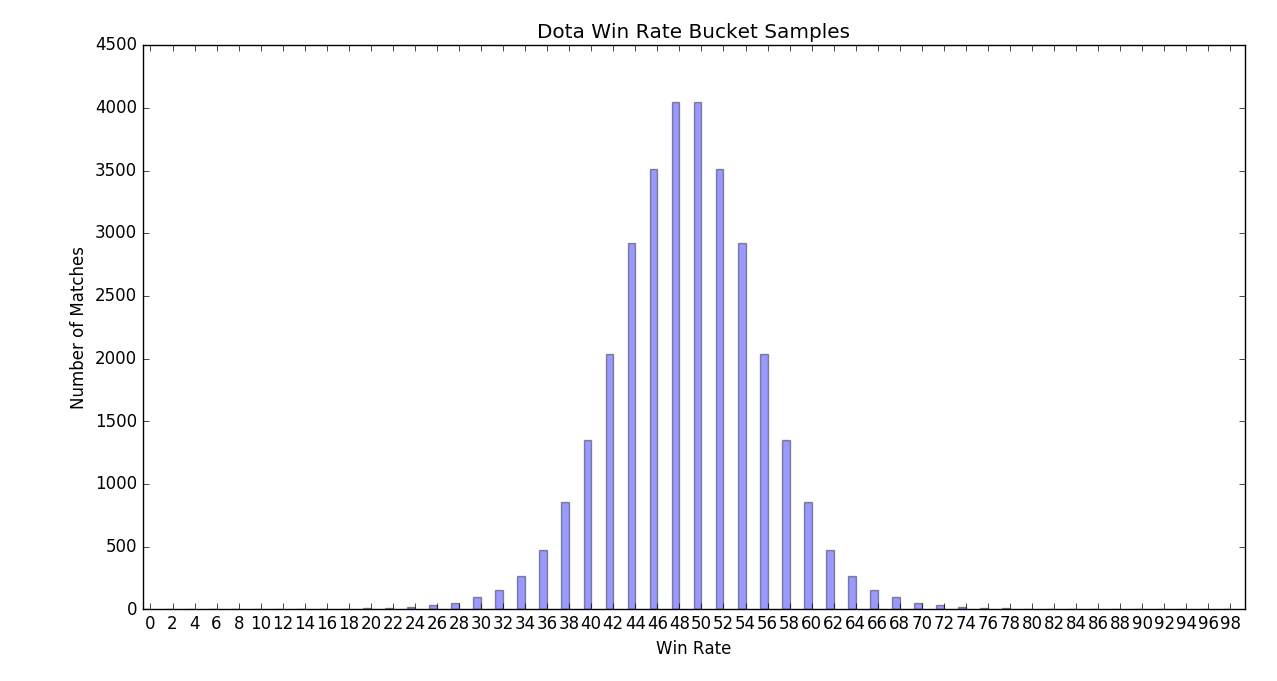
\includegraphics[width=0.45\textwidth]{result_1.png}
\caption{Match winning rate bucket sample}
\end{center}
\end{figure}

\begin{figure}[H]
\begin{center}
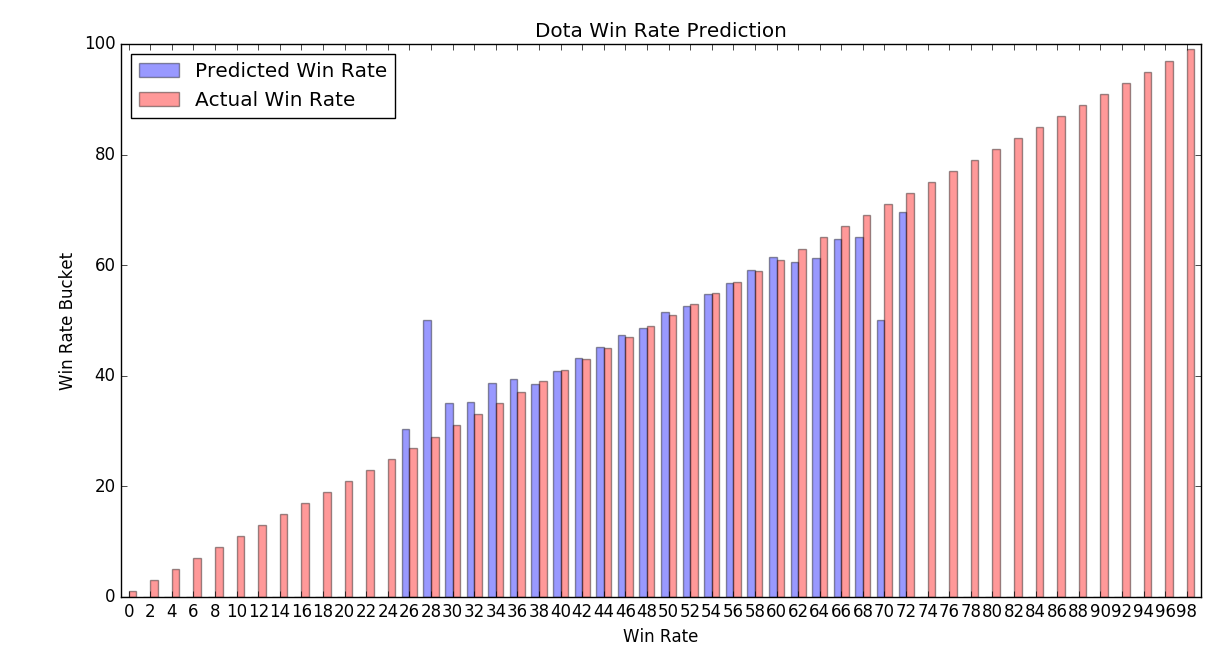
\includegraphics[width=0.45\textwidth]{result_2.png}
\caption{Primary result for winning rate prediction}
\end{center}
\end{figure}

$$\text{***UNDER CONSTRUCTION***}$$

\section{SUMMARY OF INNOVATIONS}
\begin{enumerate}
	\item Applied normal distribution as an evaluation of the difference of skill between two groups.
    \item Built a Lane Model to simplify the whole process of game into two most critical stages to reduce the complexity of analysis.
   	\item Proposed Anti \& Combo model to calculate team advantage index, which can reflect the effect of different characteristics of heroes on the result of game.
\end{enumerate}

\section{CONCLUSIONS}

$$\text{***UNDER CONSTRUCTION***}$$

\addtolength{\textheight}{-12cm}   % This command serves to balance the column lengths
                                  % on the last page of the document manually. It shortens
                                  % the textheight of the last page by a suitable amount.
                                  % This command does not take effect until the next page
                                  % so it should come on the page before the last. Make
                                  % sure that you do not shorten the textheight too much.

%%%%%%%%%%%%%%%%%%%%%%%%%%%%%%%%%%%%%%%%%%%%%%%%%%%%%%%%%%%%%%%%%%%%%%%%%%%%%%%%



%%%%%%%%%%%%%%%%%%%%%%%%%%%%%%%%%%%%%%%%%%%%%%%%%%%%%%%%%%%%%%%%%%%%%%%%%%%%%%%%



%%%%%%%%%%%%%%%%%%%%%%%%%%%%%%%%%%%%%%%%%%%%%%%%%%%%%%%%%%%%%%%%%%%%%%%%%%%%%%%%
\section*{APPENDIX}
\begin{table}[ht]
\centering
\begin{tabular}{p{2cm} p{0.6cm} p{0.6cm} p{0.4cm} p{0.4cm} p{0.6cm} p{1.0cm}}
\hline
Tasks & Y. Xu & Wang & Cao & Sun & X. Xu & Status
 \\\hline
Brainstorm & $\surd$ & $\surd$ & $\surd$ & $\surd$ & $\surd$ & Completed\\
Proposal & $\surd$ & $\surd$ & $\surd$ & $\surd$ & $\surd$ & Completed\\
Data Collection & $\surd$ &  &  & $\surd$ &  & Not Started\\
Data Clean/Integration &  & $\surd$ & $\surd$ &  & $\surd$ & Not Started\\
Algorithm Developing & $\surd$ &  &  & $\surd$ &  & Not Started\\
Data Visualization &  & $\surd$ & $\surd$ &  & $\surd$ & Not Started\\
Testing & $\surd$ & $\surd$ & $\surd$ & $\surd$ & $\surd$ & Not Started\\
\hline
\end{tabular}
\caption{Previous Tasks Assignment}
\end{table}

\begin{table}[ht]
\centering
\begin{tabular}{p{2cm} p{0.6cm} p{0.6cm} p{0.4cm} p{0.4cm} p{0.6cm} p{1.0cm}}
\hline
Tasks & Y. Xu & Wang & Cao & Sun & X. Xu & Status
 \\\hline
Brainstorm & $\surd$ & $\surd$ & $\surd$ & $\surd$ & $\surd$ & Completed\\
Proposal & $\surd$ & $\surd$ & $\surd$ & $\surd$ & $\surd$ & Completed\\
Data Collection & $\surd$ & $\surd$  &  & $\surd$ & $\surd$  & Completed\\
Data Clean/Integration & $\surd$  & & & $\surd$ & & Completed\\
Algorithm Developing & $\surd$ &  &  & $\surd$ &  & Completed\\
Data Visualization &  & $\surd$ & $\surd$ &  &  & Ongoing\\
Documents & $\surd$ & $\surd$ & & $\surd$ & & Ongoing\\
Testing & $\surd$ & $\surd$ & $\surd$ & $\surd$ & $\surd$ & Not Started\\
\hline
\end{tabular}
\caption{Current Tasks Assignment}
\end{table}


Timing Frame (Revised on Project Final Presentation section)
\begin{itemize}
\item Project Proposal (Sept.10 - Oct.17)\\
Brainstorming\\
Read related papers\\
Build Product Backlog and Sprint Backlog\\
Write a proposal.
\item Progress Report (Oct.17 - Nov.10)\\
Data Collection\\
Data Cleaning\\
Data Integration\\
Build, train models\\
Start visualization scratching
\item Project Final Presentation (Nov.11 - Dec.06)\\
Modify algorithms and improve model performance\\
Modify data visualization section\\
Prepare presentation and posters
\end{itemize}


\section*{ACKNOWLEDGMENT}

$$\text{***UNDER CONSTRUCTION***}$$



%%%%%%%%%%%%%%%%%%%%%%%%%%%%%%%%%%%%%%%%%%%%%%%%%%%%%%%%%%%%%%%%%%%%%%%%%%%%%%%%




\begin{thebibliography}{99}
\bibitem{c1} Cao C. Sports data mining technology used in basketball outcome prediction[J]. 2012.
\bibitem{c2} Kahn J. Neural network prediction of NFL football games[J]. World Wide Web electronic publication, 2003: 9-15.
\bibitem{c3} Trawinski K. A fuzzy classification system for prediction of the results of the basketball games[C], Fuzzy Systems (FUZZ), 2010 IEEE International Conference on. IEEE, 2010: 1-7.
\bibitem{c4} Buursma D. Predicting sports events from past results Towards effective betting on football matches[C], Conference Paper, presented at 14th Twente Student Conference on IT, Twente, Holland. 2011, 21.
\bibitem{c5} K. Song, T. Zhang, and C. Ma. Predicting the winning side of DotA2. tech. rep., Stanford University, 2015.
\bibitem{c6} N. Kinkade, L. Jolla, and K. Lim. DOTA 2 Win Prediction. tech. rep., University of California San Diego, 2015.
\bibitem{c7} J. Neidhardt, Y. Huang, and N. Contractor. Team vs. Team: Success Factors in a Multiplayer Online Battle Arena Game. In Academy of Management Annual Meeting Proceedings 2015(1):18725-18725, January, 2015.
\bibitem{c8} K. Conley and D. Perry. How Does He Saw Me? A Recommendation Engine for Picking Heroes in DOTA 2. CS229 Previous Projects, 2013.
\bibitem{c9} K. Kalyanaraman. To win or not to win? A Prediction Model to Determine the Outcome of a DotA2 Match. tech. rep., University of California San Diego, 2014.
\bibitem{c10} A. Drachen, M.Yancey, J.Maguire, D.Chu, I.Y.Wang, T.Mahlmann, M.Schubert, and D.Klabajan. Skill-based Differences in Spatio-temporal Team Behaviour in Defence of the Ancients 2(DotA 2). Games Media Entertainment(GEM), 2014 IEEE, vol. 2, no. dOTa 2, PP. 1-8, 2014.
\bibitem{c11} C. Eggert, M. Herrlich, J. Smeddinck, and R. Malaka. Classication of Player Roles in the Team-Based Multi-player Game Dota 2. In Entertainment Computing ICEC 2015, vol. 9353 of Lecture Notes in Computer Science, (Cham), pp. 112-125, Springer International Publishing, 2015.
\bibitem{c12} N. Pobiedina, J. Neidhardt, M. del Carmen Calatrava Moreno, and H. Werthner. Ranking Factors of Team Success. In WWW (Companion Volume), pages 1185–1194, 2013.
\bibitem{c13} N. Pobiedina, J. Neidhardt, M. D. C. C. Moreno, L. Grad-Gyenge and H. Werthner. On Successful Team Formation: Statistical Analysis of a Multiplayer Online Game. 2013 IEEE 15th Conference, In Business Informatics (CBI), (2013), pp. 55-62.
\bibitem{c14} Johansson, F. and Wikström, J., Result Prediction by Mining Replays in Dota 2, 2015.
\bibitem{c15} Dota2api (2016). Dota 2 API Documentation. [online] Available at: https://dota2api.readthedocs.io/en/latest/ [Accessed 13 Nov. 2016].
\bibitem{c16} Pandas.pydata.org. (2016). Python Data Analysis Library — pandas: Python Data Analysis Library. [online] Available at: http://pandas.pydata.org [Accessed 16 Nov. 2016].
\bibitem{c17} Drachen A, Yancey M, Maguire J, et al. Skill-based differences in spatio-temporal team behaviour in defence of the Ancients 2 (DotA 2)[C]//Games media entertainment (GEM), 2014 IEEE. IEEE, 2014: 1-8.
\bibitem{c18} Valve Corporation. (2012) The international dota2 championships official website. [Online]. Available: http://www.dota2.com/ international/overview/
\bibitem{c19} Defense of the Ancients. Wikipedia. Wikimedia Foundation, n.d. Web. 15 Nov. 2016. [Online].

\end{thebibliography}

\end{document}
